\section{Comparing to Third Party Libraries}\label{sec:comparethird}
The same experiments were conducted using \textbf{sklearn}’s implementation of these model. The same parameters were used as the first principal implementation, so to be able to compare these two. The same procedure described in Section \ref{sec:expresults} was done to gather results. The main difference between these two is the running time, the first principal implementations took the following time to finish; 21921 s (\nth{1} Experiment), 15762 s (\nth{2} Experiment), 14487 s (\nth{3} Experiment) and 13603 s (\nth{4} Experiment) while the \textbf{sklearn} implementations took; 115 s (\nth{1s} Experiment), 60 s (\nth{2} Experiment), 59 s (\nth{3} Experiment) and 54 s (\nth{4} Experiment). After some test it was noted that the implementation of the Decision Tree was the bottleneck in first principal implementation. This could be because no parallelization was used in the implementation and \textbf{sklearn}’s Decision Tree is fully implemented using \textbf{cython}. 
\begin{table}[H]
\centering
  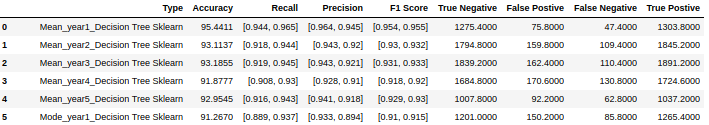
\includegraphics[scale = .65]{imgs/imp_os_skl.png}
  \caption{A snippet for results for Experiment 1 (Sklearn)}
  \label{table:imp_os_ex_skl}
\end{table}
\noindent When comparing the results shown in Table \ref{table:imp_os_ex_skl}, both first principal implementations and \textbf{sklearn} implementations seem achieve the same accuracy and F1 scores. Both of which worked better when using Mean Imputation. Although differences were noted when comparing to the average results of the forecasting periods shown in Table \ref{table:mean_metrics_skl}. It was noted that the best model when using \textbf{sklearn} was the Random Forest using only oversampled datasets (Mean Imputation) with an accuracy of 96.89\% and an F1 score of [96.9\%, 96.9\%]. When comparing this model to the first principal implementation one, there is a difference of +8.78\% in accuracy and a difference in F1 score of [+9.1\%, +8.5\%].

\noindent Unlike \textbf{sklearn} implementation the best model in the first principles implementation was the Decision Tree using only oversampled datasets (Mean Imputation). But when comparing the \textbf{sklearn} Decision tree implementation using only oversampled datasests (Mean Imputation) with the first principles implementation the differences are quite minimal when compared to the Random Forest implementation. The differences being +0.15\% in accurary and a difference of [+0.2, +0.1] in the F1 score. In both implementations the Logistic Regression had very poor results and in both implementations Feature Selection worked better than Feature Reduction.
\begin{table}[H]
\centering
  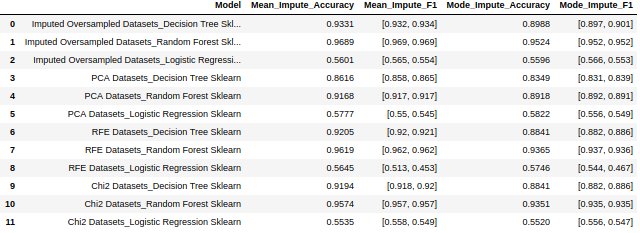
\includegraphics[scale = .7]{imgs/mean_metrics_skl.png}
  \caption{The mean results (forecasting periods) for each Experiment (Sklearn)}
  \label{table:mean_metrics_skl}
\end{table}
\noindent In this implementation the best predicted forecasting period was \nth{1} year using Mean Imputation. This is the same best forecasting period achieved when using the first principles implementation. The difference being that it was achieved using Random Forest rather than Decision Tree. The plots for this forecasting period can be shown in Figure \ref{fig:pp_plots_results_skl}. When comparing the confusion matrix with the confusion matrix shown in Figure \ref{fig:pp_plots_results} there is a difference of +93.28 for True Positive, -95.6 for False Positive, -31.92 for False Negative, +32.92. Although this difference in performance shows that this best model is better than the best model of the first principal the differences are minor when using such metric. 
\noindent Comparing both ROC curves of the best forecasting period as described above there is a difference of +0.04 in AUC which again is very low. The ROC curves can be shown in Figure \ref{fig:pp_plots_results_skl} (\textbf{sklearn}) and Figure \ref{fig:pp_plots_results} (first principles).

\noindent So to summarize the main differences between the third party library and the first principle implementation is the execution time and the best performing model which is Random Forest in \textbf{sklearn} and Decision Trees in first principle implementation. Altought the best model is different all accuracies and F1 scores are in general similiar to each other. 
\begin{figure}[H]
\centering
  \begin{subfigure}[b]{0.5\textwidth}
    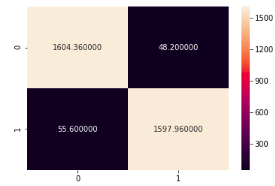
\includegraphics[scale = .7]{imgs/confusion_matrix_2.png}
    \caption{Confusion Matrix}
  \label{fig:confusion_matrix_skl}
  \end{subfigure}
  %
  \begin{subfigure}[b]{0.4\textwidth}
    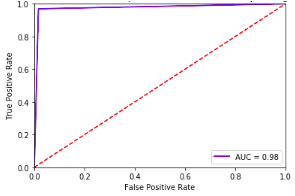
\includegraphics[scale = .9]{imgs/rf_mean_imp_yr1_skl.png}
  \caption{ROC curve}
  \label{fig:roc_skl}
  \end{subfigure}
  \caption{Plots for best performing Model (Random Forest) using best imputation technique (Mean); Confusion Matrix using averaged values of all forecasting periods and ROC curve for best forecasting period (\nth{1} Year) using \textbf{sklearn}}
  \label{fig:pp_plots_results_skl}
\end{figure}


